\subsubsection*{Konqueror und Nautilus}
Linuxer, welche die Dateimanager Konqueror (KDE) oder Nautilus (Gnome) nutzen, k�nnen das Verstecken und Extrahieren auch mit wenigen Mausklicks erledigen:

\begin{itemize}
 \item Das Konqueror/Dolphin Servicemen� f�r steghide gibt es bei KDE-apps.org. Nach dem Download ist das Archiv zu entpacken. Die .desktop-Datei kopiert man nach \textit{\$HOME/.kde/share/apps/konqueror/servicemenus/} und das Shell-Script nach \textit{/usr/local/bin}. Download: \href{http://kde-look.org/content/show.php?content=105172}{http://kde-look.org/content/show.php?content=105172}\\

\begin{figure}[htb]
\begin{center}
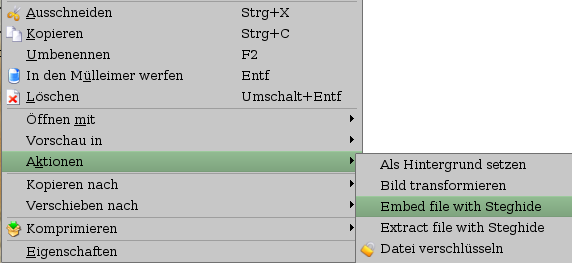
\includegraphics[scale=0.5]{../screenshots/steghide_kde.png}
\caption{Steghide Men� im Konqueror}
\label{abb:steghide_kde}
\end{center}
\end{figure}

In Zukunft findet man bei einem Rechtsklick auf die Cover-Datei (JPEG, WAV, AU) im Untermen� \textit{Aktionen} die Men�punkte f�r das Einf�gen und Extrahieren von Dateien mit \textit{steghide}. (Bild \ref{abb:steghide_kde}). F�r das Verstecken (embed) w�hlt man noch eine zweite Datei, die dann nach Abfrage des Passworts in der Cover-Datei versteckt wird.

\item Das \href{http://www.trademarkclan.net/files/steghide_jpg.tar.gz}{Nautilus Action Script} ist ebenfalls zu entpacken und in \$HOME/gnome2/nautilus-scripts zu speichern.\\

Dann mit der rechten Maustaste auf eine JPEG-Datei klicken, den Men�punkt ``Scripte - steghide\_jpg'' w�hlen und den Anweisungen folgen.
\end{itemize}
